\documentclass[11pt]{article}

\usepackage[T1]{fontenc}
\usepackage[utf8]{inputenc}
\usepackage{amsmath,amssymb,amsthm,mathtools}
\usepackage{booktabs}
\usepackage{graphicx}
\usepackage[margin=1in]{geometry}
\usepackage{microtype}
\usepackage[numbers,sort&compress]{natbib}
\usepackage{xcolor}
\usepackage[colorlinks=true,allcolors=blue!55!black]{hyperref}

\definecolor{bodytext}{HTML}{111111}
\definecolor{panelgray}{HTML}{F2F4F7}
\pagecolor{white}
\color{bodytext}

\newtheorem{theorem}{Theorem}
\newtheorem{proposition}{Proposition}
\newtheorem{corollary}{Corollary}
\newtheorem{lemma}{Lemma}
\theoremstyle{remark}
\newtheorem{remark}{Remark}

\newcommand{\Matern}{\mathcal M}
\newcommand{\E}{\mathbb E}
\newcommand{\R}{\mathbb R}
\newcommand{\tr}{\operatorname{tr}}
\newcommand{\KL}{D_{\mathrm{KL}}}

\title{How Local Averaging Moves Mat\'ern Pairwise Range Targets:\\
A Smoothness-Dependent Phase Law}
\author{Sasha Cui\\Independent researcher}
\date{Draft of \today}

\begin{document}
\maketitle

\begin{abstract}
Spatial measurements often represent local averages, but are subsequently fitted
as if they were point observations.  This changes the population target of
covariance estimation, not merely its finite-sample bias.  We study a stationary
Mat\'ern Gaussian field in \(\R^d\), observed through a known compact symmetric
averaging kernel of bandwidth \(h\).  For a fixed nonzero-lag Gaussian two-point
likelihood with fixed known smoothness \(\nu\), we characterize the exact
pseudo-variance and pseudo-decay and derive their small-support expansions.  The
naive decay shift is
of order \(h^{2\nu}\) for \(0<\nu<1\), \(h^2\log(1/h)\) at \(\nu=1\), and
\(h^2\) for \(\nu>1\).  Explicit coefficients show that, for every \(\nu>0\)
and any nondegenerate compact symmetric kernel, naive point-support fitting
underestimates inverse range---and therefore overestimates spatial range---for
all sufficiently small \(h\).  The coefficient for \(\nu>1\) remains positive
for anisotropic averaging kernels.  A support-aware covariance propagates both
the field and measurement noise through the observation operator and removes
the population shift when the operator and fixed nuisance parameters are
correctly specified.  Deterministic two-dimensional quadrature verifies the
three rate regimes, while synthetic finite-grid likelihood experiments
illustrate discrete, irregular, and boundary behavior.  The result isolates a
concrete inferential cost of ignored spatial support while making no novelty
claim for the standard change-of-support covariance formula itself.
\end{abstract}

\section{Introduction}

Spatial values recorded on pixels, grid cells, administrative regions, or after
kernel preprocessing are local aggregates of an underlying field.  The
change-of-support literature models such observations by integrating the latent
process over their supports \citep{gelfand2001support,chacon2024change}.  In
practice, however, smoothed values are often assigned to declared centers and a
point-support covariance is fitted.  Relative to the latent parameters, this is
a support-misinterpreted model.  A single two-point covariance can still be
matched exactly by different variance and decay parameters; a multi-lag
likelihood is genuinely misspecified and selects a Kullback--Leibler (KL)
projection \citep{bachoc2018misspecified}.

That qualitative conclusion is familiar, but it does not answer three basic
questions.  How fast does the target move as the support shrinks?  Does the rate
depend on Mat\'ern smoothness?  Is the direction of the range error stable across
dimension and averaging kernels?  These questions matter because the Mat\'ern
covariance changes regularity at the origin as \(\nu\) crosses one.  A symmetric
kernel cancels first-order Taylor terms at nonzero lags, but it cannot cancel a
cusp or fractional power at the origin.

Temporal aggregation of autoregressive and Ornstein--Uhlenbeck models is
classical \citep{amemiya1972aggregation,stram1986aggregation}, and integrated
Ornstein--Uhlenbeck inference has been studied directly
\citep{folia2018aggregated}.  Consequently, a one-dimensional exponential
calculation alone is not a novelty claim.  Reviews and geostatistical methods
for incompatible supports establish the block-to-block covariance and
area-to-point prediction problems
\citep{gotway2002incompatible,kyriakidis2005areal}.  Most closely,
\citet{fuentes2007approximate} constructs a likelihood for block averages in
terms of an underlying point covariance and studies a Mat\'ern example.  That
work correctly models the support; it does not derive the pseudo-range selected
when block averages are instead treated as points.  Generic misspecified-GP KL
theory \citep{bachoc2018misspecified} supplies the projection framework but not
the support-specific coefficient or sign.  Our contribution is the explicit
all-smoothness, \(d\)-dimensional fixed-lag pseudo-parameter expansion.  In
particular:

\begin{enumerate}
  \item We derive a phase law for the naive Mat\'ern decay target: orders
  \(h^{2\nu}\), \(h^2\log(1/h)\), and \(h^2\) in the rough, threshold, and
  smooth regimes.
  \item We give explicit coefficients.  Origin expansions, together with a
  Bessel-function identity in the smooth regime, prove that normalized
  correlation increases, hence inverse range decreases, for every \(\nu>0\)
  and any compact symmetric kernel when \(h\) is sufficiently small.
  \item We distinguish the continuous interior theorem from discrete,
  row-normalized, and boundary-truncated smoothing.  We then compute finite-grid
  full-likelihood KL targets and compare naive and support-aware fits using only
  synthetic data.
\end{enumerate}

The covariance transformation \(S K S^\top\), block kriging, generic KL
projection under misspecification, and temporal aggregation are prior work; they
are not claimed as contributions.  Recent finite-grid Mat\'ern likelihood work
also treats discretization and edge effects without studying the target induced
by a preprocessing smoother \citep{simons2026finite}.  Our narrower focus is the
smoothness-dependent target displacement caused by ignoring observation support.

\section{Model and pseudo-target}

\subsection{Latent field and local support}

Let \(Y=\{Y(t):t\in\R^d\}\) be a mean-zero stationary Gaussian field with

\begin{equation}
  \operatorname{Cov}\{Y(t),Y(t+r)\}
  = C(r)=v\Matern_\nu(\alpha\lVert r\rVert),
  \qquad v>0,\quad \alpha>0,\quad \nu>0,
  \label{eq:matern-covariance}
\end{equation}
where

\begin{equation}
  \Matern_\nu(x)
  =\frac{2^{1-\nu}}{\Gamma(\nu)}x^\nu K_\nu(x),
  \qquad \Matern_\nu(0)=1.
  \label{eq:matern-correlation}
\end{equation}

Thus \(\alpha\) is an inverse range; larger \(\alpha\) means shorter dependence.
This convention must not be mixed with the common length-scale parameterization
\(\alpha=\sqrt{2\nu}/\ell\).

Let \(k\) be a symmetric probability density supported on
\(B(0,L)\subset\R^d\), let \(k_h(u)=h^{-d}k(u/h)\), and define the mean-square
convolution

\begin{equation}
  Z_h(t)=\int_{\R^d} k_h(u)Y(t-u)\,du.
  \label{eq:smoothed-field}
\end{equation}

If \(U,V\stackrel{\mathrm{iid}}{\sim}k\) and \(D=U-V\), stationarity and Fubini's
theorem give the exact smoothed covariance

\begin{equation}
  C_h(r)
  =v\E\!\left[\Matern_\nu\{\alpha\lVert r+hD\rVert\}\right].
  \label{eq:smoothed-covariance}
\end{equation}

Write

\begin{equation}
  \Sigma_k=\E(UU^\top),\quad T_k=\tr(\Sigma_k),\quad
  m_q=\E\lVert D\rVert^q,
  \label{eq:kernel-moments}
\end{equation}
so that \(m_2=2T_k\).  We assume \(T_k>0\).

\subsection{Naive Gaussian pair fit}

Fix \(r=Re\), with \(R>0\) and \(\lVert e\rVert=1\).  The smoothed pair has
variance \(C_h(0)\) and correlation

\begin{equation}
  \rho_h(r)=\frac{C_h(r)}{C_h(0)}.
\end{equation}

A naive point-support model with the correct known \(\nu\) but unknown variance
and decay uses covariance

\begin{equation}
  v^\dagger
  \begin{pmatrix}
    1 & \Matern_\nu(\alpha^\dagger R)\\
    \Matern_\nu(\alpha^\dagger R) & 1
  \end{pmatrix}.
  \label{eq:naive-pair}
\end{equation}

The true two-by-two covariance belongs to this family.  Therefore its Gaussian
KL minimizer is exactly

\begin{equation}
  v_h^\dagger=C_h(0),
  \qquad
  \Matern_\nu(\alpha_h^\dagger R)=\rho_h(r).
  \label{eq:exact-pseudo-target}
\end{equation}

Existence follows from \(0<\rho_h(r)<1\) for \(r\ne0\).  Positivity follows
from \(k\geq0\) and \(\Matern_\nu>0\).  Strict inequality follows because the
smoothed field has spectral density
\(\lvert\widehat k(h\omega)\rvert^2 f_\nu(\omega)\), which is positive on a
neighborhood of the origin, while \(e^{i\omega^\top r}\) is not identically one
there.  Uniqueness follows from

\begin{equation}
  \Matern_\nu'(x)
  =-\frac{2^{1-\nu}}{\Gamma(\nu)}x^\nu K_{\nu-1}(x)<0,
  \qquad x>0.
  \label{eq:matern-derivative}
\end{equation}

For completeness, consider a fixed lattice, a lag \(r\) belonging to that
lattice, and increasing rectangular F{\o}lner domains.  If the parameter space
is compact, the target is unique and interior, correlations are bounded away
from one, and the pair log likelihood is continuous with an integrable
quadratic envelope, the ergodic theorem gives the uniform law needed for
pair-composite consistency at \((v_h^\dagger,\alpha_h^\dagger)\).  Overlapping
pairs are dependent, so uncertainty requires a Godambe or long-run covariance,
not an independence Hessian.  We do not use fixed-domain asymptotics to claim
separate consistency of variance and range; such a claim would conflict with
Mat\'ern microergodicity results
\citep{zhang2004inconsistent,stein1999interpolation}.

\section{Small-support phase law}

For \(z=\alpha R\), define the directional kernel variance
\(a_k(e)=e^\top\Sigma_k e\) and

\begin{equation}
  B_{\nu,k}(r)
  =\alpha^2\left[
    a_k(e)\Matern_\nu''(z)
    +\{T_k-a_k(e)\}\frac{\Matern_\nu'(z)}{z}
  \right].
  \label{eq:B-definition}
\end{equation}

\begin{proposition}[Fixed nonzero lag]
For \(r\) in a compact annulus bounded away from zero and
\(h\leq \lVert r\rVert/(4L)\),
\begin{equation}
  \frac{C_h(r)}{v}
  =\Matern_\nu(\alpha\lVert r\rVert)
  +h^2 B_{\nu,k}(r)+O(h^4).
  \label{eq:fixed-lag-expansion}
\end{equation}
The remainder is uniform when \(\alpha\) also ranges over a compact subset of
\((0,\infty)\).
\end{proposition}

The variance behaves differently because the Mat\'ern function is expanded at
the origin.  Put

\begin{equation}
  c_\nu
  =-\frac{\Gamma(-\nu)}{2^{2\nu}\Gamma(\nu)}
  =\frac{\Gamma(1-\nu)}{\nu 2^{2\nu}\Gamma(\nu)}>0,
  \qquad 0<\nu<1.
\end{equation}

\begin{theorem}[Mat\'ern support phase law]
Fix \(\nu>0\).  Under the preceding assumptions, as \(h\downarrow0\),
\begin{align}
  \frac{C_h(0)}{v}
  & =1-c_\nu m_{2\nu}(\alpha h)^{2\nu}+O(h^2),
  &&0<\nu<1,\label{eq:variance-rough}\\
  \frac{C_h(0)}{v}
  & =1-\frac{m_2}{2}(\alpha h)^2\log\{1/(\alpha h)\}+O(h^2),
  &&\nu=1,\label{eq:variance-threshold}\\
  \frac{C_h(0)}{v}
  & =1-\frac{m_2}{4(\nu-1)}(\alpha h)^2+o(h^2),
  &&\nu>1.\label{eq:variance-smooth}
\end{align}

Moreover, the naive decay target in \eqref{eq:exact-pseudo-target} satisfies
\begin{align}
  \alpha_h^\dagger-\alpha
  & =
  \frac{\Matern_\nu(z)c_\nu m_{2\nu}\alpha^{2\nu}}
       {R\Matern_\nu'(z)}h^{2\nu}
  +O\!\left(h^{\min(4\nu,2)}\right),
  &&0<\nu<1,\label{eq:decay-rough}\\
  \alpha_h^\dagger-\alpha
  & \sim
  \frac{m_2\Matern_1(z)\alpha^2}
       {2R\Matern_1'(z)}h^2\log(1/h),
  &&\nu=1,\label{eq:decay-threshold}\\
  \alpha_h^\dagger-\alpha
  & =\frac{A_{\nu,k}(r)}{R\Matern_\nu'(z)}h^2+\mathcal R_\nu(h),
  &&\nu>1,\label{eq:decay-smooth}
\end{align}
where
\begin{align}
  A_{\nu,k}(r)
  &=\alpha^2\{(2\nu-2)a_k(e)+T_k\}G_\nu(z)>0,\\
  G_\nu(z)
  &=\frac{\Matern_\nu(z)}{2\nu-2}
    +\frac{\Matern_\nu'(z)}{z}
   =\frac{2^{1-\nu}}{\Gamma(\nu)}
     \frac{z^\nu K_{\nu-2}(z)}{2\nu-2}>0,
  \label{eq:G-positive}
\end{align}
and \(\mathcal R_\nu(h)=O(h^{2\nu})\) for \(1<\nu<2\),
\(O\{h^4\log(1/h)\}\) for \(\nu=2\), and \(O(h^4)\) for \(\nu>2\).
For fixed \(\nu\), these remainders are uniform for \(\alpha\) in a compact
subset of \((0,\infty)\) and \(r\) in a compact annulus bounded away from zero.
They are not uniform as \(\nu\) approaches one or two.
\end{theorem}

Every leading coefficient in
\eqref{eq:decay-rough}--\eqref{eq:decay-smooth} is negative because
\(\Matern_\nu'(z)<0\).  Thus, for sufficiently small positive \(h\),

\begin{equation}
  v_h^\dagger<v,\qquad
  \rho_h(r)>\Matern_\nu(\alpha R),\qquad
  \alpha_h^\dagger<\alpha.
  \label{eq:sign-conclusion}
\end{equation}

The naive model overestimates range.  The result does not require an isotropic
smoother: anisotropy enters only through \(a_k(e)\) and \(T_k\), whose combination
in \eqref{eq:G-positive} remains positive.  For an isotropic kernel with
\(\Sigma_k=\sigma_k^2I_d\),

\begin{equation}
  A_{\nu,k}(r)=\sigma_k^2\alpha^2(2\nu+d-2)G_\nu(z).
\end{equation}

\begin{remark}[Why symmetry does not imply an \(h^2\) bias]
Symmetry removes the order-\(h\) term at a fixed nonzero lag.  When
\(0<\nu<1\), however, the origin expansion contains \(\lVert r\rVert^{2\nu}\),
which changes the variance at order \(h^{2\nu}\).  Normalizing by that variance
dominates the order-\(h^2\) off-diagonal change.  At \(\nu=1\), the origin term is
\(h^2\log(1/h)\).  Only for \(\nu>1\) do ordinary second derivatives control
both pieces.
\end{remark}

\begin{remark}[The fitted lag is fixed]
The expansion holds for \(R\) bounded away from zero.  If \(R=ch\), the
nonzero-lag Taylor expansion is no longer uniform and the relative target
displacement need not vanish.  No shrinking-lag conclusion is claimed.
\end{remark}

\section{Support-aware finite-grid likelihood}

The continuous theorem concerns translation-invariant interior averaging.  The
finite experiment starts from raw sites
\(X_{\mathrm{in}}=(x_1,\ldots,x_n)\) and a rectangular row-stochastic operator
\(S_h\in\R^{m\times n}\).  If independent measurement noise is present before
smoothing,

\begin{equation}
  y=S_h\{Y(X_{\mathrm{in}})+\epsilon\},
  \qquad \epsilon\sim N(0,\tau^2I_n),
\end{equation}
then the correct covariance is

\begin{equation}
  \Sigma_{\mathrm{corr}}(\alpha)
  =S_h\{K_\alpha(X_{\mathrm{in}},X_{\mathrm{in}})+\tau^2I_n\}S_h^\top.
  \label{eq:corrected-covariance}
\end{equation}

The naive declared-center point-support model instead uses

\begin{equation}
  \Sigma_{\mathrm{naive}}(\alpha)
  =K_\alpha(X_{\mathrm{out}},X_{\mathrm{out}})+\tau^2I_m.
  \label{eq:naive-covariance}
\end{equation}

Besides ignoring support, \eqref{eq:naive-covariance} incorrectly treats
pre-smoothing noise as independent post-smoothing noise.  With variance,
smoothness, and nugget fixed at their generating values, the finite-design
population target minimizes

\begin{equation}
  Q_n(\alpha)
  =\frac12\left[
    \log\det\Sigma(\alpha)
    +\tr\{\Sigma(\alpha)^{-1}\Sigma_0\}
  \right],
  \label{eq:finite-kl}
\end{equation}
where constants independent of \(\alpha\) are omitted.  The corrected family
contains \(\Sigma_0\) exactly, provided the known operator and fixed nuisance
parameters are correct and \(\alpha\) is identifiable on the finite design;
the naive family generally does not.  Our primary support-only experiment sets
\(\tau=0\), preventing noise timing from confounding the support effect.  A
separate combined-misspecification run with \(\tau^2=0.05\) is retained as a
reproducibility stress artifact but is not used for the principal claims.

A rectangular \(S_h\) is intentional.  If a square parameter-independent
smoother is invertible, the exact transformed likelihood is merely a change of
coordinates and need not lose information.  Rectangular aggregation represents
the scientifically relevant reduction from raw locations to fewer supported
measurements.

Boundary row normalization is not covered by the interior theorem.  For two
location-dependent scaled kernels with means \(\mu_s\) and \(\mu_t\), a direct
fixed-lag expansion gives
\begin{equation}
  C_{h,s,t}(r)
  =C(r)+h\nabla C(r)^\top(\mu_s-\mu_t)+O(h^2).
  \label{eq:boundary-first-order}
\end{equation}
A truncated kernel can therefore introduce an order-\(h\) term and destroy
stationarity.  The interior theorem provides no universal boundary sign.  We
report one boundary-retaining and one fixed jittered design as illustrations,
not as a boundary scaling study.

\section{Synthetic validation}

\subsection{Continuous two-dimensional quadrature}

We used a product Epanechnikov density

\begin{equation}
  k(u)=\prod_{j=1}^d\frac34(1-u_j^2)\mathbf 1\{|u_j|\leq1\}.
\end{equation}

The one-dimensional density of \(U_j-V_j\) is available in closed form, so
tensor Gauss--Legendre quadrature evaluates \eqref{eq:smoothed-covariance}
deterministically.  We used \(d=2\), \(\alpha=R=1\), quadrature order 96 per
coordinate, 18 geometrically spaced bandwidths from 0.003 to 0.3, and
\(\nu\in\{0.25,0.5,0.75,1,1.5,2.5\}\).  For each cell we solved
\eqref{eq:exact-pseudo-target} by monotone root finding.  Repeating the entire
grid at quadrature orders 64 and 128 changed pseudo-decay by at most
\(4.4\times10^{-8}\) and \(5.2\times10^{-9}\), respectively, relative to
order 96.

All 108 computed decay shifts \(\alpha-\alpha_h^\dagger\) were positive.  An
ordinary least-squares slope over the six smallest bandwidths on log--log axes
was 0.515, 0.999, and 1.468 for \(\nu=0.25,0.5,0.75\), compared with theoretical
powers 0.5, 1, and 1.5.  At \(\nu=1\), the raw slope was 1.817, as expected from
the logarithmic modifier rather than a pure power.  The slopes for
\(\nu=1.5\) and 2.5 were 1.994 and 2.000.  Figure~\ref{fig:phase} displays the
full paths and the coefficient-level theorem comparison.  At the smallest
bandwidth, exact-shift to leading-term ratios were 1.021, 1.000, 0.958, 1.059,
0.997, and 1.000 in increasing order of \(\nu\).

\begin{figure}[t]
  \centering
  \IfFileExists{figures/phase_law.pdf}{
    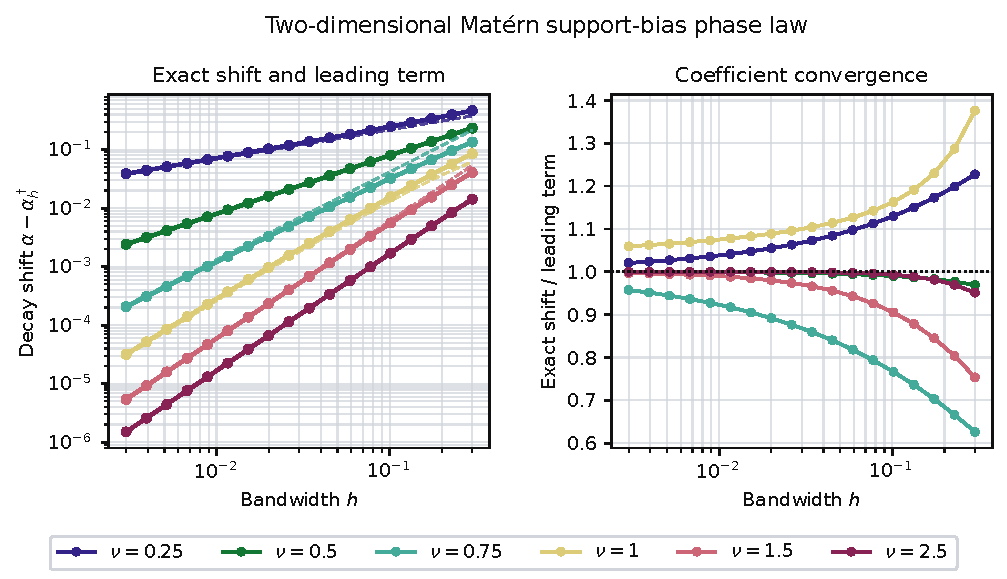
\includegraphics[width=0.92\linewidth]{figures/phase_law.pdf}
  }{
    \fcolorbox{black}{panelgray}{\parbox[c][2.0in][c]{0.86\linewidth}{
      \centering Figure generated after the reproducible analysis step.}}
  }
  \caption{Continuous two-dimensional pseudo-decay shift under product
  Epanechnikov smoothing.  Left: exact shifts (solid) and theorem leading terms
  with their explicit coefficients (dashed).  Right: their ratio, which
  approaches one as \(h\downarrow0\).}
  \label{fig:phase}
\end{figure}

\subsection{Finite-grid full likelihood}

The core design uses a \(19\times19\) input lattice with spacing 0.25 and every
second location as a candidate output center.  Interior outputs are trimmed by
0.75 in each coordinate.  We set \(v=\alpha=1\), \(\tau^2=0\),
\(\nu\in\{0.5,1,1.5,2.5\}\), and
\(h\in\{0,0.3,0.5,0.7\}\).  Radial Epanechnikov rows are normalized exactly.
The zero-bandwidth operator is an exact rectangular selector.  Stress panels
retain boundary centers, perturb each input coordinate uniformly in
\([-0.04,0.04]\) before clipping to the original bounding box, and examine
one-dimensional increasing-domain lattices with 100, 225, and 400 raw sites.
The irregular panel uses one fixed jitter realization.

For each configuration, the finite-design population criterion is minimized by
bounded scalar optimization over
\(\log\alpha\in[\log(0.02),\log(5)]\).  Replicate likelihoods are evaluated on
a 161-point equally spaced log-decay profile; an interior grid minimum is
refined by three-point quadratic interpolation, while an endpoint minimum is
retained as a boundary fit.  Gaussian raw-observation vectors with the declared
covariance are transformed by \(S_h\).  Configurations sharing all parameters
except \(h\) reuse standard-normal draws.  No numerical jitter is added.  A
Cholesky or population-optimization failure aborts its configuration and makes
the reducer mark the run incomplete; no such failure occurred.

% FINITE_RESULTS_START
The promoted study used 200 replicates in each of 21 configurations, producing
8,400 fitted estimates.  The reducer verified configuration hashes, row counts,
and unique model--replicate keys for every task shard.  Independent checks also
verified finite numerical fields, expected model labels, replicate indices, and
metadata.
Across the 16 core two-dimensional configurations, the corrected population
target differed from the true decay by at most \(1.3\times10^{-7}\).  At the
largest bandwidth, \(h=0.7\), the naive population targets were 0.152, 0.414,
0.573, and 0.740 for \(\nu=0.5,1,1.5,2.5\), respectively.  Their corresponding
Monte Carlo means were 0.151, 0.407, 0.570, and 0.738; the corrected means were
1.090, 0.990, 0.990, and 0.994.  The comparatively noisy corrected estimate at
\(\nu=0.5\) nevertheless remained within two Monte Carlo standard errors of its
population target.

No optimizer or covariance failure was discarded.  Six of the 6,400 core fits
landed at the declared bounds, and those fits remain in Figure~\ref{fig:finite}
and Table~\ref{tab:finite}.  Including boundary outputs changed both the output
dimension and the rough-field naive target, from 0.152 to 0.135 at \(h=0.7\);
for the fixed jittered design the target changed from 0.289 to 0.284 at
\(h=0.5\).  In both stress cases the corrected target
remained one.  In the one-dimensional domain-growth check, increasing the
number of raw sites from 100 to 400 reduced the corrected estimator standard
deviation from 0.529 to 0.177 and the naive standard deviation from 0.151 to
0.068, while at \(n=400\) their means remained within 0.026 and 0.009,
respectively, of their population targets
(Figure~\ref{fig:convergence}).
% FINITE_RESULTS_END

\begin{figure}[t]
  \centering
  \IfFileExists{figures/finite_targets.pdf}{
    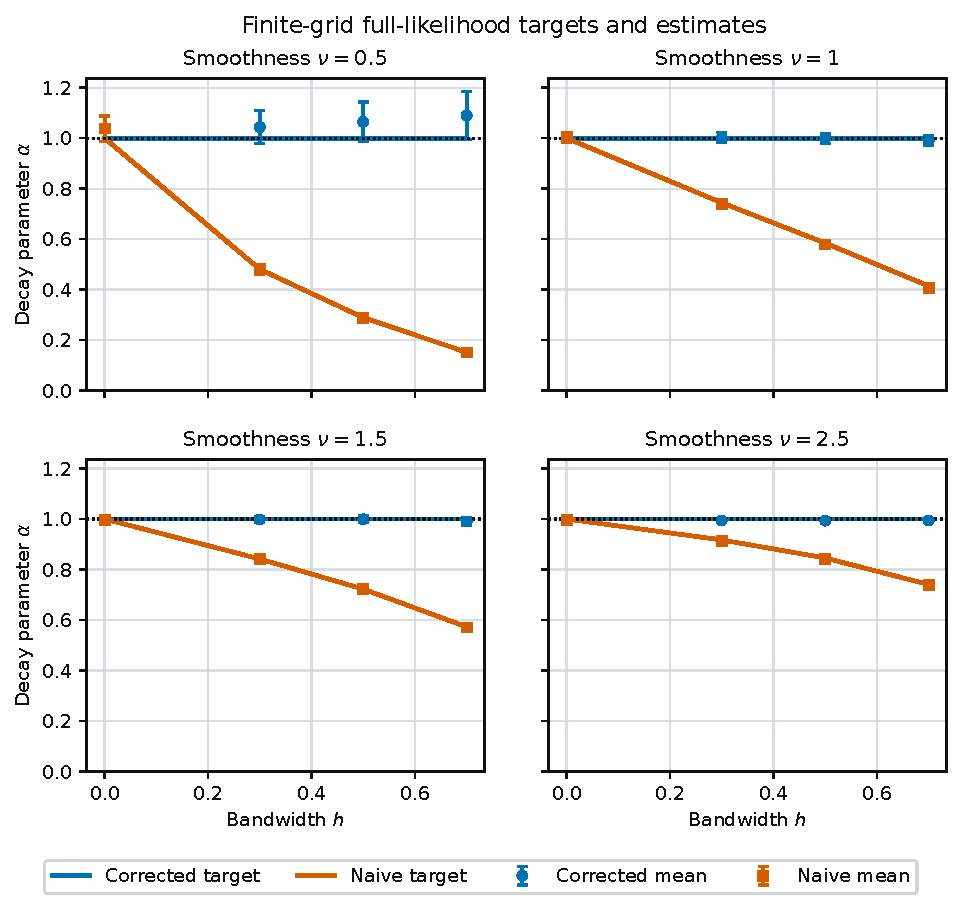
\includegraphics[width=0.96\linewidth]{figures/finite_targets.pdf}
  }{
    \fcolorbox{black}{panelgray}{\parbox[c][2.0in][c]{0.88\linewidth}{
      \centering Figure generated after the promoted synthetic run.}}
  }
  \caption{Finite-design population targets and Monte Carlo mean decay estimates
  for corrected and naive likelihoods.  Error bars show two Monte Carlo standard
  errors of the mean, not estimator confidence intervals.}
  \label{fig:finite}
\end{figure}

\begin{figure}[t]
  \centering
  \IfFileExists{figures/finite_convergence.pdf}{
    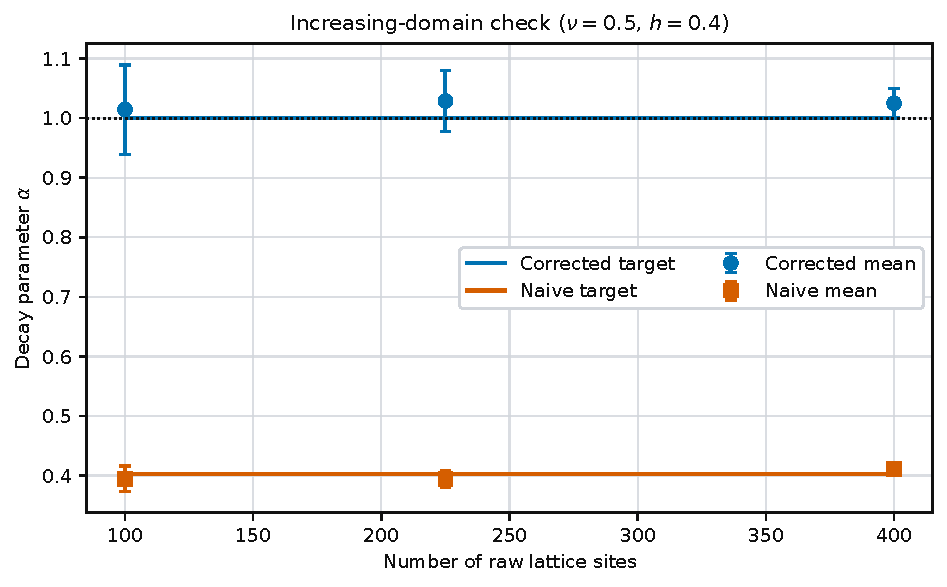
\includegraphics[width=0.88\linewidth]{figures/finite_convergence.pdf}
  }{
    \fcolorbox{black}{panelgray}{\parbox[c][1.8in][c]{0.82\linewidth}{
      \centering Figure generated after the promoted synthetic run.}}
  }
  \caption{Increasing-domain check for the finite-grid likelihood.  Lines are
  nonrandom finite-design targets and points are Monte Carlo means from 200
  replicates; error bars show two Monte Carlo standard errors of each mean.}
  \label{fig:convergence}
\end{figure}

\begin{table}[t]
  \centering
  \caption{Finite-design validation at \(h=0.7\).  The table is generated from
  immutable task shards; no failed or boundary-hitting fit is silently removed.}
  \label{tab:finite}
  \IfFileExists{tables/finite_summary.tex}{
    \begin{tabular}{llrrrr}
\toprule
$\nu$ & Model & Target & Mean & MCSE & Bound hits\\
\midrule
0.5 & Corrected & 1.000 & 1.090 & 0.047 & 3\\
0.5 & Naive & 0.152 & 0.151 & 0.004 & 0\\
1 & Corrected & 1.000 & 0.990 & 0.010 & 0\\
1 & Naive & 0.414 & 0.407 & 0.005 & 0\\
1.5 & Corrected & 1.000 & 0.990 & 0.007 & 0\\
1.5 & Naive & 0.573 & 0.570 & 0.005 & 0\\
2.5 & Corrected & 1.000 & 0.994 & 0.004 & 0\\
2.5 & Naive & 0.740 & 0.738 & 0.003 & 0\\
\bottomrule
\end{tabular}

  }{
    \begin{tabular}{lrrr}
      \toprule
      Model & Population target & Mean estimate & Boundary fits\\
      \midrule
      Corrected & --- & --- & ---\\
      Naive & --- & --- & ---\\
      \bottomrule
    \end{tabular}
  }
\end{table}

\section{Discussion}

The theorem separates two effects that are often conflated.  Linear propagation
of covariance through a known support is standard.  The new object here is the
parameter selected when that propagation is ignored.  For rough Mat\'ern fields,
the origin singularity makes the pseudo-target move at a fractional power of
bandwidth.  For smooth fields, a Bessel recurrence shows that the combined
variance and nonzero-lag correction still increases normalized correlation,
including under anisotropic smoothing.

Several limitations define the scope of the result.  First, \(\nu\) and the
support are treated as known.  Jointly estimating smoothness, bandwidth, variance,
and range may be weakly identified.  Second, the closed target is for a
two-point composite fit.  A full likelihood cannot generally match every
smoothed lag; its KL target is computed numerically in our finite designs.
Third, fixed-resolution discrete averaging does not converge to continuous
convolution merely because the spatial domain grows.  A mixed-domain quadrature
limit or an exact discrete-weight theorem is required.  Fourth, boundary
normalization creates location-dependent supports and can introduce first-order
terms.  Fifth, the synthetic study fixes nuisance parameters so that it tests the
central target-shift mechanism rather than a larger optimization problem.

These restrictions are preferable to an unsupported broad claim.  They also
suggest direct extensions: a uniform discrete-to-continuous approximation,
joint nuisance profiling, spectral full-likelihood expansions, and explicit
boundary counterexamples.  Without such extensions, the present contribution is
best viewed as a focused methodological paper rather than a high-dimensional
statistics result.

\section{Conclusion}

For a fixed nonzero-lag pair fit under translation-invariant interior
averaging, ignored support makes a Mat\'ern field look more persistent than it
is.  The magnitude is controlled by smoothness: \(h^{2\nu}\),
\(h^2\log(1/h)\), or \(h^2\).  A support-aware observation covariance removes
the finite-design population shift when the operator is known, nuisance
parameters are correctly specified, and decay is identifiable.  The result
provides a theorem-level diagnostic for when preprocessing is negligible and
when it changes the pairwise range estimand; it makes no universal claim for
boundary supports or arbitrary full-likelihood fits.

\appendix
\section{Proof of the phase theorem}

\begin{proof}

Let \(f_\alpha(x)=\Matern_\nu(\alpha\lVert x\rVert)\).  Since \(r\) is bounded
away from zero and \(D\) is bounded, a fourth-order Taylor expansion is uniform.
Because \(D=U-V\) has a centrally symmetric law, both
\(\E D=0\) and \(\E(D^{\otimes3})=0\); moreover
\(\E(DD^\top)=2\Sigma_k\).  Therefore

\begin{equation}
  \E f_\alpha(r+hD)
  =f_\alpha(r)
   +\frac{h^2}{2}\tr\{\nabla^2f_\alpha(r)\E(DD^\top)\}
   +O(h^4).
\end{equation}

For \(r=Re\),

\begin{equation}
  \nabla^2f_\alpha(r)
  =\alpha^2\Matern_\nu''(z)ee^\top
   +\alpha^2\frac{\Matern_\nu'(z)}{z}(I-ee^\top),
\end{equation}
which proves \eqref{eq:fixed-lag-expansion}.

For noninteger \(\nu\), the origin expansion is

\begin{equation}
  \Matern_\nu(x)
  =\sum_{j=0}^{\infty}
    \frac{(x^2/4)^j}{j!(1-\nu)_j}
   +\frac{\Gamma(-\nu)}{2^{2\nu}\Gamma(\nu)}x^{2\nu}
    \sum_{j=0}^{\infty}
    \frac{(x^2/4)^j}{j!(1+\nu)_j}.
  \label{eq:bessel-series}
\end{equation}

Taking expectations at \(x=\alpha h\lVert D\rVert\) yields
\eqref{eq:variance-rough} and \eqref{eq:variance-smooth}.  At \(\nu=1\),

\begin{equation}
  \Matern_1(x)
  =1+\frac{x^2}{2}
    \{\log(x/2)+\gamma_{\mathrm E}-1/2\}
   +O\{x^4(1+|\log x|)\},
\end{equation}
which proves \eqref{eq:variance-threshold}.

At the second transition,
\begin{equation}
  \Matern_2(x)
  =1-\frac{x^2}{4}
   +x^4\left\{\frac{3}{64}
   -\frac{\log(x/2)+\gamma_{\mathrm E}}{16}\right\}
   +O\{x^6(1+|\log x|)\}.
\end{equation}
This gives an \(O\{h^4\log(1/h)\}\) variance remainder at \(\nu=2\).
For fixed \(\nu>2\), four-times differentiability at the origin gives
\[
  \Matern_\nu(x)
  =1-\frac{x^2}{4(\nu-1)}+O(x^4).
\]
For \(1<\nu<2\), the fractional term in
\eqref{eq:bessel-series} is \(O(x^{2\nu})\).

Divide the fixed-lag expansion by the relevant variance expansion and apply a
first-order Taylor expansion to the inverse of
\(\alpha\mapsto\Matern_\nu(\alpha R)\).  This directly gives
\eqref{eq:decay-rough} and \eqref{eq:decay-threshold}; the same division and
inverse expansion preserve the stated \(O(h^{2\nu})\),
\(O\{h^4\log(1/h)\}\), and \(O(h^4)\) remainders in the three smooth
subregimes.  For \(\nu>1\), the
order-\(h^2\) coefficient of normalized correlation is

\begin{equation}
  B_{\nu,k}(r)
  +\Matern_\nu(z)\frac{\alpha^2m_2}{4(\nu-1)}.
\end{equation}

The Mat\'ern correlation satisfies

\begin{equation}
  \Matern_\nu''(z)
  +\frac{1-2\nu}{z}\Matern_\nu'(z)
  -\Matern_\nu(z)=0.
\end{equation}

Using \(m_2=2T_k\), the coefficient becomes
\(A_{\nu,k}(r)\).  Finally,

\begin{equation}
  K_\nu(z)=K_{\nu-2}(z)+\frac{2(\nu-1)}{z}K_{\nu-1}(z)
\end{equation}

implies \eqref{eq:G-positive}.  Positivity of \(K_\eta(z)\) for real \(\eta\)
and \(z>0\), together with \eqref{eq:matern-derivative}, proves the sign.
\end{proof}

\section{Exact exponential benchmark}

For \(d=1\), \(\nu=1/2\), and the Epanechnikov density
\(k(u)=\tfrac34(1-u^2)\mathbf 1\{|u|\leq1\}\), the density of \(D=U-V\) is

\begin{equation}
  g(w)=\frac35-\frac34|w|^2+\frac38|w|^3-\frac{3}{160}|w|^5,
  \qquad |w|\leq2.
\end{equation}

With \(x=\alpha h\), define

\begin{equation}
  s(x)=\E e^{-x|D|},\qquad
  M_k(x)=\E e^{xU}=\frac{3(x\cosh x-\sinh x)}{x^3},\qquad
  q(x)=M_k(x)^2.
\end{equation}

Then \(C_h(0)=v s(x)\), and for \(R\geq2h\),

\begin{equation}
  C_h(R)=vq(x)e^{-\alpha R}.
\end{equation}

The exact naive pair target is

\begin{equation}
  v_h^\dagger=vs(x),\qquad
  \alpha_h^\dagger
  =\alpha-\frac1R\log\frac{q(x)}{s(x)}.
\end{equation}

For \(x>0\), compact support and nondegeneracy give
\[
  1<q(x)/s(x)<e^{2x}.
\]
Indeed, condition on \(A=|U|\) and \(B=|V|\), and put
\(p=A+B\) and \(m=|A-B|\).  Symmetry of the signs gives conditional
numerator and denominator proportional to
\(\cosh(xp)+\cosh(xm)\) and \(e^{-xp}+e^{-xm}\), respectively.
The lower inequality follows from \(\cosh(t)\geq e^{-t}\), with strictness
off \(A=B=0\).  Since \(p+m=2\max(A,B)\leq2\),
\(\cosh(xp)<e^{xp}\leq e^{2x-xm}\) and
\(\cosh(xm)\leq e^{xm}\leq e^{2x-xp}\), with strictness on a set of
positive probability.  Averaging proves the upper inequality.
Since \(R\geq2h\), this implies
\(0<\alpha-R^{-1}\log\{q(x)/s(x)\}<\alpha\).  Variance and decay are
therefore both strictly underestimated.  The small-bandwidth expansions are

\begin{align}
  s(x)&=1-\frac{18}{35}x+\frac15x^2-\frac4{63}x^3
        +\frac3{175}x^4+O(x^5),\\
  q(x)&=1+\frac15x^2+\frac3{175}x^4+O(x^6),\\
  \log\{q(x)/s(x)\}&=\frac{18}{35}x+\frac{162}{1225}x^2+O(x^3).
\end{align}

This benchmark is used as an exact software regression test, not as the paper's
novelty claim.

\section{Reproducibility contract}

The public code at
\url{https://github.com/Sasha-Cui/HighDimSpatialStatistics} is archived for
this draft under the immutable tag \texttt{paper-draft-v0.1.0}.  It uses an
immutable JSON manifest, SHA-256 configuration hashes,
deterministic seed derivation, one task-local atomic shard, and an
\texttt{afterany} reducer that refuses to mark a run complete when a shard is
missing or invalid.  The zero-bandwidth selector, row sums, row rank, corrected
population target, grid interpolation, and closed exponential formulas are unit
tested.  The reported implementation adds no adaptive diagonal jitter.  All
paper figures and tables are regenerated from audited aggregate CSV files.

\bibliographystyle{plainnat}
\bibliography{references}

\end{document}
